\section{Introdução}
\label{sec:introducao}

\begin{figure}[t]
\centering
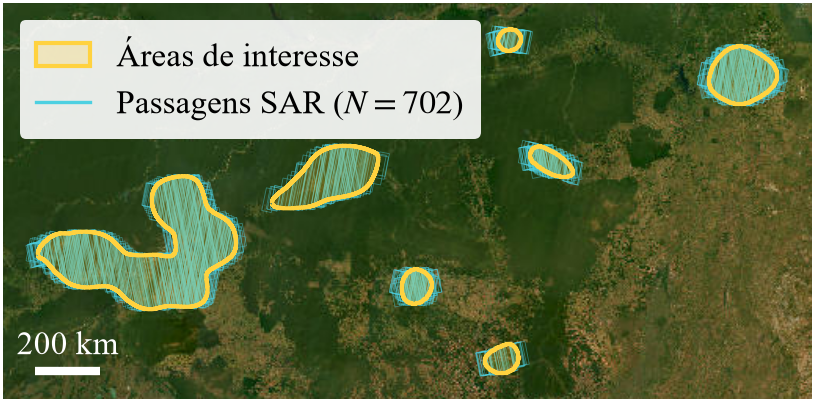
\includegraphics[width=\columnwidth]{area_estudo}
\caption{Áreas de interesse e contornos das 702 passagens SAR candidatas. Imagem de fundo: Esri World Imagery.}
\label{fig:area}
\end{figure}

O monitoramento da Amazônia por sensores ópticos é limitado pela cobertura frequente de nuvens~\cite{asner2001}, o que favorece os sensores de radar de abertura sintética (SAR), capazes de imagear através delas~\cite{moreira2013}. Com as constelações de pequenos satélites SAR, as oportunidades de aquisição sobre uma mesma região se multiplicam, mas as faixas imageadas se sobrepõem e cada aquisição tem custo. O problema é, então, escolher um subconjunto de passagens que cubra as áreas de interesse com poucas aquisições e pouca sobreposição. Com $N$ passagens candidatas, há $2^N$ subconjuntos possíveis; trata-se de uma variante do problema de cobertura de conjuntos, que é NP-difícil~\cite{karp1972}, o que motiva o uso de meta-heurísticas como o algoritmo genético (AG)~\cite{beasley1996}.

Neste trabalho, consideram-se sete áreas de interesse na Amazônia, que somam cerca de 210~mil~km$^2$, e $N = 702$ passagens candidatas da constelação ICEYE, em banda X e modo \textit{Stripmap}, previstas entre 14 de junho e 15 de agosto de 2023 (Fig.~\ref{fig:area}). As faixas são muito redundantes: se todas fossem adquiridas, cada ponto das áreas seria imageado, em média, 12,8 vezes.

O objetivo é aplicar um AG a esse problema e comparar, pelas curvas de convergência e pela aptidão final, (a)~os métodos de seleção por roleta, torneio e ranking, (b)~diferentes taxas de cruzamento e mutação e (c)~a execução com e sem elitismo. O desempenho do AG depende diretamente dessas escolhas~\cite{eiben1999}.
